
%%%%%%%%%%%%%%%%%%%%%%% file typeinst.tex %%%%%%%%%%%%%%%%%%%%%%%%%
%
% This is the LaTeX source for the instructions to authors using
% the LaTeX document class 'llncs.cls' for contributions to
% the Lecture Notes in Computer Sciences series.
% http://www.springer.com/lncs       Springer Heidelberg 2006/05/04
%
% It may be used as a template for your own input - copy it
% to a new file with a new name and use it as the basis
% for your article.
%
% NB: the document class 'llncs' has its own and detailed documentation, see
% ftp://ftp.springer.de/data/pubftp/pub/tex/latex/llncs/latex2e/llncsdoc.pdf
%
%%%%%%%%%%%%%%%%%%%%%%%%%%%%%%%%%%%%%%%%%%%%%%%%%%%%%%%%%%%%%%%%%%%


\documentclass[runningheads,a4paper]{llncs}

\usepackage{amssymb}
\setcounter{tocdepth}{3}
\usepackage{graphicx}

\usepackage{url}
\urldef{\mailsa}\path|{alfred.hofmann, ursula.barth, ingrid.haas, frank.holzwarth,|
\urldef{\mailsb}\path|anna.kramer, leonie.kunz, christine.reiss, nicole.sator,|
\urldef{\mailsc}\path|erika.siebert-cole, peter.strasser, lncs}@springer.com|    
\newcommand{\keywords}[1]{\par\addvspace\baselineskip
\noindent\keywordname\enspace\ignorespaces#1}

\begin{document}

\mainmatter  % start of an individual contribution

% first the title is needed
\title{Lecture Notes in Computer Science:\\Authors' Instructions
for the Preparation\\of Camera-Ready
Contributions\\to LNCS/LNAI/LNBI Proceedings}

% a short form should be given in case it is too long for the running head
\titlerunning{Lecture Notes in Computer Science: Authors' Instructions}

% the name(s) of the author(s) follow(s) next
%
% NB: Chinese authors should write their first names(s) in front of
% their surnames. This ensures that the names appear correctly in
% the running heads and the author index.
%
\author{Alfred Hofmann%
\thanks{Please note that the LNCS Editorial assumes that all authors have used
the western naming convention, with given names preceding surnames. This determines
the structure of the names in the running heads and the author index.}%
\and Ursula Barth\and Ingrid Haas\and Frank Holzwarth\and\\
Anna Kramer\and Leonie Kunz\and Christine Rei\ss\and\\
Nicole Sator\and Erika Siebert-Cole\and Peter Stra\ss er}
%
\authorrunning{Lecture Notes in Computer Science: Authors' Instructions}
% (feature abused for this document to repeat the title also on left hand pages)

% the affiliations are given next; don't give your e-mail address
% unless you accept that it will be published
\institute{Springer-Verlag, Computer Science Editorial,\\
Tiergartenstr. 17, 69121 Heidelberg, Germany\\
\mailsa\\
\mailsb\\
\mailsc\\
\url{http://www.springer.com/lncs}}

%
% NB: a more complex sample for affiliations and the mapping to the
% corresponding authors can be found in the file "llncs.dem"
% (search for the string "\mainmatter" where a contribution starts).
% "llncs.dem" accompanies the document class "llncs.cls".
%

\toctitle{Lecture Notes in Computer Science}
\tocauthor{Authors' Instructions}
\maketitle


\begin{abstract}
The abstract should summarize the contents of the paper and should
contain at least 70 and at most 150 words. It should be written using the
\emph{abstract} environment.
\keywords{We would like to encourage you to list your keywords within
the abstract section}
\end{abstract}


\section{Background: Compressed Text Indexes}

You are strongly encouraged to use \LaTeXe{} for the
preparation of your camera-ready manuscript together with the
corresponding Springer class file \verb+llncs.cls+. Only if you use
\LaTeXe{} can hyperlinks be generated in the online version
of your manuscript.

The \LaTeX{} source of this instruction file for \LaTeX{} users may be
used as a template. This is
located in the ``authors'' subdirectory in
\url{ftp://ftp.springer.de/pub/tex/latex/llncs/latex2e/instruct/} and
entitled \texttt{typeinst.tex}. There is a separate package for Word 
users. Kindly send the final and checked source
and PDF files of your paper to the Contact Volume Editor. This is
usually one of the organizers of the conference. You should make sure
that the \LaTeX{} and the PDF files are identical and correct and that
only one version of your paper is sent. It is not possible to update
files at a later stage. Please note that we do not need the printed
paper.

\subsubsection{Burrows-Wheeler Transform.}
The Burrows-Wheeler Transform of a string is a reversible permutation of its characters that was originally developed for compression because it tends to cluster together identical symbols, so it can be efficiently stored with techniques such as run-length encoding or move-to-front coding. More recently, it has been applied to full-text indexing because it allows the search of a substring in large texts in linear time with respect to the length of the substring, with a small memory footprint. The BWT of a string $T=t_1t_2 \ldots t_n$ is constructed by sorting its $n$ cyclic shifts $t_1t_2 \ldots t_n$, $t_2 \ldots t_n t_1$, \ldots,  $t_n t_1 \ldots t_{n-1}$ in lexicographic order. The matrix obtained is called the Burrows-Wheeler matrix and the sequence from its last column is the BWT. An example is given below. The last character $t_n$ is always a unique terminating symbol $\$$ that is lexicographically smaller than all the symbols in $T$ and is essential for decoding. Storing the first and last column of the BWM is sufficient for finding the number of exact matches of a query in $T$. For locating the position of the matches in $T$ an additional data structure is required, the suffix array. 

\subsubsection{Suffix Arrays.} The suffix array of a string $T$ is an array of integers that provides the starting position of $T$'s suffixes, after they have been ordered lexicographically. Formally, if $T_{i,j}$ is the substring $t_i t_{i+1} \ldots t_j$ of $T$ and SA is the suffix array of $T$, then $T_{SA[1],n}<T_{SA[2],n}<\ldots <T_{SA[n],n}$. It is related to the BWT, since looking at the substrings preceding the terminating character $\$$ in the BWM rows gives the suffixes of $T$ in lexicographical order. In fact, the BWT can be derived in linear time from the suffix array by looping through its values and recording the character occurring just before each suffix in the original text, i.e. $BWT[i]=T[SA[i]-1]$ if $SA[i]\neq1$ and $BWT[i]=\$$ if $SA[i]=1$. The suffix array coupled with the BWT and two additional data structures form the FM-index, which enables the backward search of a pattern in text.

\subsubsection{Backward search}
Any occurrence of a pattern $P$ in text is a prefix for some suffix of $T$, so all occurrences will be adjacent in the suffix array of $T$, since suffixes starting with $P$ are sorted together in a SA-interval. The backward search starts with the last character of $P$ and successively extends it to longer suffixes, calculating their SA-intervals, until the SA-interval of the entire query is reached. Let $C[a]$ be the total number of occurences in $T$ of characters smaller than $a$ in the alphabet, the $C$-array essentially representing the first column of the BWM. Then if $P'$ is a suffix of the query $P$ and $[l(P'),r(P')]$ is its corresponding SA-interval, then the search can be extended to $aP'$ by calculating the new SA-interval:
\newline
\begin{equation} 
l(aP')=C[a]+rank_{BWT}(a,l(P')-1)+1 
\end{equation} 

\begin{equation} 
r(aP')=C[a]+rank_{BWT}(a,r(P))
\end{equation}

The search starts with the SA-interval of the empty string, $[1,n]$ and successively adds one character of $P$ in backward order. When the search is completed, it returns a SA-interval $[l,r]$ for the entire query $P$. If $r \geq l$, there are $r-l+1$ matches for $P$ and their locations in $T$ are given by $SA[i]$ for $l \leq i \leq r$. Otherwise, the pattern does not exist in $T$. If the $C$-array and the ranks have already been stored, the backward search can be performed in $O(|P|)$ time in strings with DNA alphabet.

\subsubsection{Wavelet Trees}
As the alphabet of a string contains more symbols, rank queries become more computationally expensive since they scale linearly with the alphabet size. The wavelet tree is a data structure designed to store strings with large alphabets efficiently and provide rank calculations in logarithmic time. A wavelet tree converts a string into a balanced binary-tree of bitvectors, whose root is built by taking the sorted alphabet and replacing the lower half of smaller symbols with a 0, and the other half of larger symbols with a 1 in the string. This creates ambiguity initially, but at each tree level, each half of the parent node's alphabet is re-split into 2 and re-encoded, so the ambiguity lessens as the tree is traversed in depth. At the leaves, there is no ambiguity at all. The tree is defined recursively as follows: take the lexicographically ordered alphabet, split it into 2 equal halves; in the string corresponding to the current node (start with original string at root), replace the first half of letters with 0 and the other half with 1; the left child node will contain the 0-encoded symbols and the right child node will contain the 1-encoded symbols, preserving their order from the original string; reapply the first step for each child node recursively until the alphabet left in each node contains only one or two symbols (so a 0 or 1 determines which symbol it is). An example is given in the figure below.

 \begin{figure}
\centering
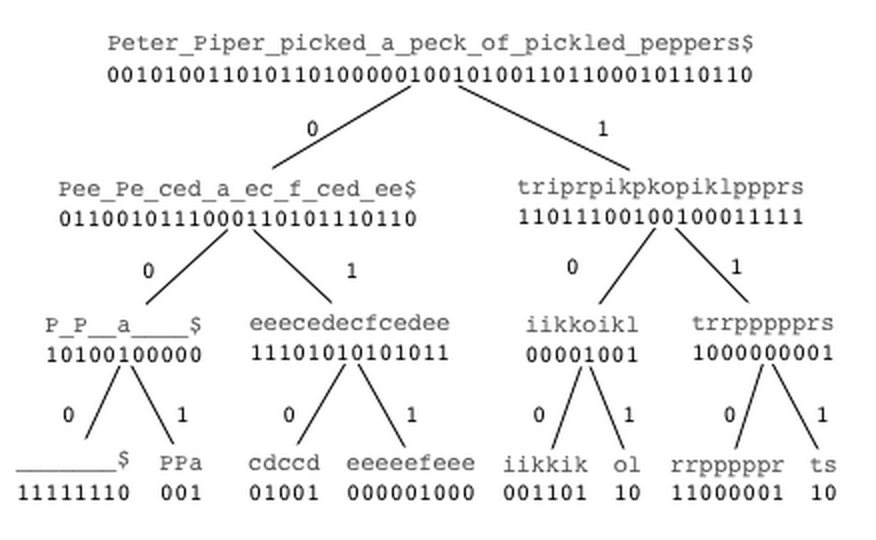
\includegraphics[height=5cm]{wt}
\caption{Bla}
\label{fig:wt}
\end{figure}

In order to answer a rank query over the original string with large alphabet, repeated rank queries over the bitvectors in the wavelet tree nodes are used as a guide to the right subtree that contains the leaf where the queried symbol is non-ambiguously encoded. The rank of the queried symbol in this leaf is equal to its rank in the original string. The number of rank queries needed to reach the leaf is equal to the height of the tree, i.e. $\log_{2} {|\Sigma|}$ if we let $\Sigma$ be the set of symbols in the alphabet. Computing ranks over binary vectors can be done in constant time, so a rank query in a wavelet tree-encoded string has complexity $O(\log_{2} {|\Sigma|})$. Next, we will show how the data structures described in this section can be used to store variation inside a reference genome in a way that supports read mapping.

\section{Encoding a variation-aware reference structure}

We propose a linear PRG conceptually equivalent with a directed, acyclic, partial order graph, that is generated from a reference sequence and a set of alternative sequences at given variation loci. The graph is linearised into a long string over an alphabet extended with new symbols marking the variants, for which the FM-index can be constructed. Building this data structure requires multiple steps. 
\begin{enumerate}
\item First, homologous regions of shared sequence between the input reference genomes must be identified. These must be of size $k$ at least (where $k$ is pre-defined), and will act like anchors for the coordinates of the variation sites. 
\item Second, for any locus between two anchor regions, the set of possible haplotypes must be determined from the input genomes, but they do not need to be aligned. Indels are naturally supported by haplotypes of different lengths.
\item Each variation locus is assigned two unique numeric identifiers, one even and one odd. The odd identifiers will mark locus boundaries and the even identifiers will mark alternative allele boundaries.
\item For each variation locus, its left anchor is added to the linear PRG, followed by its odd identifier. Then each sequence coming from that locus, starting with the reference sequence, is successively added to the linear PRG, followed by the even locus identifier, except the last sequence, which is followed by the odd identifier.
\item Convert the linear PRG to integer alphabet (A->1,C->2,G->3,T->4, variation locus identifiers->5,6,...)
\item The FM-index (suffix array, BWT, wavelet tree over BWT) of the linear PRG is constructed and we will call this the vBWT.
\end{enumerate}

An illustration of these steps on a toy example is given in Figure.

\begin{figure}
\centering
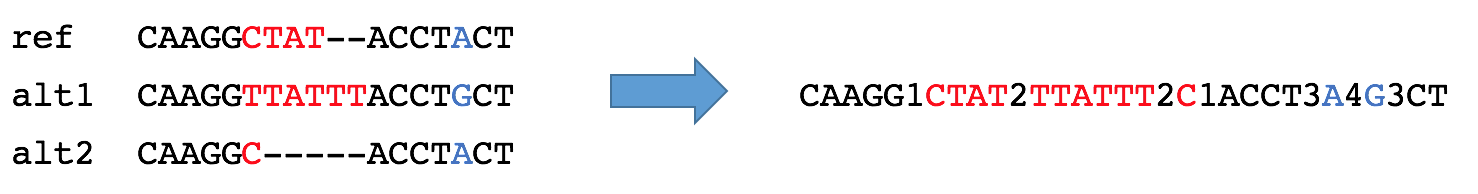
\includegraphics[height=1.5cm]{linPRG}
\caption{Bla}
\label{fig:example}
\end{figure}


This vBWT construction allows reads to be mapped to it through a modified backward search algorithm. The variation markers that surround homologous alleles prevent wrong alignment across their boundaries and ensure the right path is taken when a read crosses a region with multiple alternative sequences. Since these markers are unique to each variation site, we can locate the beginning and end of a site in the Burrows-Wheeler matrix after the permutation of the linear PRG string. This enables reads to cross site junctions and map to the linear PRG when they span multiple sites of variation, allowing for new recombinations of known haplotypes. It also makes the method potentially adjustable for long reads. More importantly, the markers force the ends of alternative sequences coming from the same site to be sorted together in a separate block in the Burrows-Wheeler matrix, even if they do not have high sequence similarity. Therefore, homologous alleles from each site can be queried concurrently instead of looping through every one of them and checking if they match the read, which would happen if the markers were the same for all sites and non-homologous alleles got mixed up. 

The linear PRG preserves information about the variant locations, so its coordinates can be projected back onto the primary reference sequence, enabling the integration with functional annotations and standard file formats. A path through the linear PRG is a string obtained by traversing the linear PRG and concatenating the non-variable segments with one sequence from each site that contains variation. If the first sequence is chosen from all variation sites, then the standard reference genome is obtained. Otherwise, a new alternative reference is obtained that can be used with usual software for downstream variant calling analysis. Our goal is to use the linear PRG mapping to genotype each of the variation sites, then use the link information from reads spanning multiple sites to phase adjacent variants and hence infer a personalised reference that corresponds to the path that is closest to the sample analysed.

\section{Exact mapping}
In this section, we present a modified backward search algorithm for exact matching against the vBWT that is aware of alternative sequence paths. When reads align to the non-variable part of of the linear PRG or when a variant locus is long enough to enclose the entire read, the usual backward search algorithm can be used. Otherwise, when the read must cross variation site junctions in order to align, site identifiers and some alternative alleles must be ignored by the search. This means a read can align to multiple substrings of the linear PRG that may not be adjacent in the BWM, so the search can return multiple SA-intervals. This is illustrated in figure. 

At each step in backward search, before extending to the next character, we need to check whether the current matched read substring is preceded by a variation marker anywhere in the linear PRG. A scan for symbols larger than 4 must be performed in the BWT within the range given by the current SA-interval (need to explain range search 2d in a wavelet tree). If a variation marker is found and it is an odd number, the read is about cross a site boundary, i.e. is about to walk in or walk out of a site. The suffix array can be queried to find the position of the two odd numbers in the liner PRG: the number occurring at a smaller position will mark the beginning of site and the other one will mark the end of site. If the search cursor is next to the start of the site, it is just the site marker that needs to be skipped so the SA-interval (size 1) of the suffix starting with that marker needs to be added to the set of intervals that will be extended with the next character in the read. If the search cursor is next to the end of a site, all alternative alleles from that site need to be queried. Their ends are sorted together in the BWM because of the markers, so they can be queried concurrently by adding the SA-interval of suffixes starting with all numbers marking that site (even and odd). 

If the variation marker found is an even number, the read is about to cross an allele boundary, which means its current suffix matches the beginning of an alternative allele and the read is about to walk out of a site, so the search cursor needs to jump to the start of site. As previously described, the odd markers corresponding to that site can be found in the sorted first column of the BWM, and then querying the suffix array decides which one marks the start of site. Then the SA-interval (size 1) for the BWM row starting with this odd marker is recorded.

Once the check for variation markers is finished and all candidate SA-intervals have been added, each interval can be extended with the next character in the read by using equations 1 and 2.

\subsubsection{Headings.}

Headings should be capitalized
(i.e., nouns, verbs, and all other words
except articles, prepositions, and conjunctions should be set with an
initial capital) and should,
with the exception of the title, be aligned to the left.
Words joined by a hyphen are subject to a special rule. If the first
word can stand alone, the second word should be capitalized.

Here are some examples of headings: ``Criteria to Disprove
Context-Freeness of Collage Language", ``On Correcting the Intrusion of
Tracing Non-deterministic Programs by Software", ``A User-Friendly and
Extendable Data Distribution System", ``Multi-flip Networks:
Parallelizing GenSAT", ``Self-determinations of Man".

\subsubsection{Lemmas, Propositions, and Theorems.}

The numbers accorded to lemmas, propositions, and theorems, etc. should
appear in consecutive order, starting with Lemma 1, and not, for
example, with Lemma 11.

\subsection{Figures}

For \LaTeX\ users, we recommend using the \emph{graphics} or \emph{graphicx}
package and the \verb+\includegraphics+ command.

Please check that the lines in line drawings are not
interrupted and are of a constant width. Grids and details within the
figures must be clearly legible and may not be written one on top of
the other. Line drawings should have a resolution of at least 800 dpi
(preferably 1200 dpi). The lettering in figures should have a height of
2~mm (10-point type). Figures should be numbered and should have a
caption which should always be positioned \emph{under} the figures, in
contrast to the caption belonging to a table, which should always appear
\emph{above} the table; this is simply achieved as matter of sequence in
your source.

Please center the figures or your tabular material by using the \verb+\centering+
declaration. Short captions are centered by default between the margins
and typeset in 9-point type (Fig.~\ref{fig:example} shows an example).
The distance between text and figure is preset to be about 8~mm, the
distance between figure and caption about 6~mm.

To ensure that the reproduction of your illustrations is of a reasonable
quality, we advise against the use of shading. The contrast should be as
pronounced as possible.

If screenshots are necessary, please make sure that you are happy with
the print quality before you send the files.
\begin{figure}
\centering
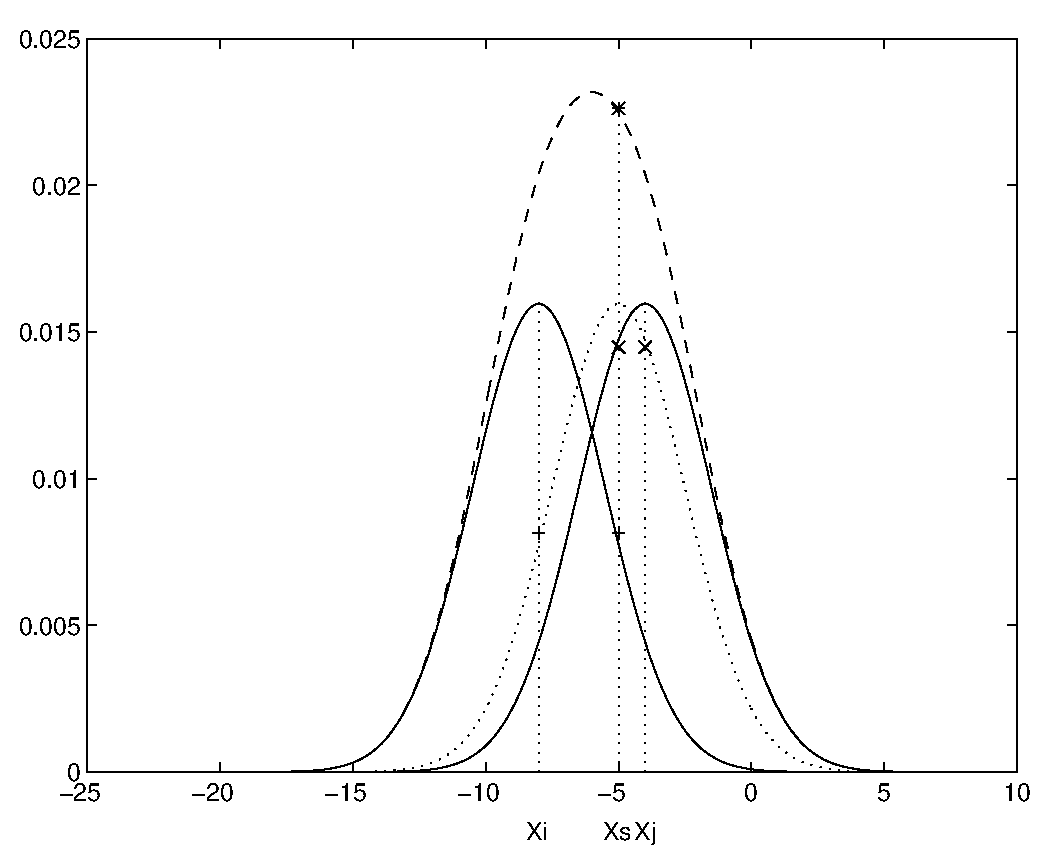
\includegraphics[height=6.2cm]{eijkel2}
\caption{One kernel at $x_s$ (\emph{dotted kernel}) or two kernels at
$x_i$ and $x_j$ (\textit{left and right}) lead to the same summed estimate
at $x_s$. This shows a figure consisting of different types of
lines. Elements of the figure described in the caption should be set in
italics, in parentheses, as shown in this sample caption.}
\label{fig:example}
\end{figure}

Please define figures (and tables) as floating objects. Please avoid
using optional location parameters like ``\verb+[h]+" for ``here".

\paragraph{Remark 1.}

In the printed volumes, illustrations are generally black and white
(halftones), and only in exceptional cases, and if the author is
prepared to cover the extra cost for color reproduction, are colored
pictures accepted. Colored pictures are welcome in the electronic
version free of charge. If you send colored figures that are to be
printed in black and white, please make sure that they really are
legible in black and white. Some colors as well as the contrast of
converted colors show up very poorly when printed in black and white.

\subsection{Formulas}

Displayed equations or formulas are centered and set on a separate
line (with an extra line or halfline space above and below). Displayed
expressions should be numbered for reference. The numbers should be
consecutive within each section or within the contribution,
with numbers enclosed in parentheses and set on the right margin --
which is the default if you use the \emph{equation} environment, e.g.,
\begin{equation}
  \psi (u) = \int_{o}^{T} \left[\frac{1}{2}
  \left(\Lambda_{o}^{-1} u,u\right) + N^{\ast} (-u)\right] dt \;  .
\end{equation}

Equations should be punctuated in the same way as ordinary
text but with a small space before the end punctuation mark.

\subsection{Footnotes}

The superscript numeral used to refer to a footnote appears in the text
either directly after the word to be discussed or -- in relation to a
phrase or a sentence -- following the punctuation sign (comma,
semicolon, or period). Footnotes should appear at the bottom of
the
normal text area, with a line of about 2~cm set
immediately above them.\footnote{The footnote numeral is set flush left
and the text follows with the usual word spacing.}

\subsection{Program Code}

Program listings or program commands in the text are normally set in
typewriter font, e.g., CMTT10 or Courier.

\medskip

\noindent
{\it Example of a Computer Program}
\begin{verbatim}
program Inflation (Output)
  {Assuming annual inflation rates of 7%, 8%, and 10%,...
   years};
   const
     MaxYears = 10;
   var
     Year: 0..MaxYears;
     Factor1, Factor2, Factor3: Real;
   begin
     Year := 0;
     Factor1 := 1.0; Factor2 := 1.0; Factor3 := 1.0;
     WriteLn('Year  7% 8% 10%'); WriteLn;
     repeat
       Year := Year + 1;
       Factor1 := Factor1 * 1.07;
       Factor2 := Factor2 * 1.08;
       Factor3 := Factor3 * 1.10;
       WriteLn(Year:5,Factor1:7:3,Factor2:7:3,Factor3:7:3)
     until Year = MaxYears
end.
\end{verbatim}
%
\noindent
{\small (Example from Jensen K., Wirth N. (1991) Pascal user manual and
report. Springer, New York)}

\subsection{Citations}

For citations in the text please use
square brackets and consecutive numbers: \cite{jour}, \cite{lncschap},
\cite{proceeding1} -- provided automatically
by \LaTeX 's \verb|\cite| \dots\verb|\bibitem| mechanism.

\subsection{Page Numbering and Running Heads}

There is no need to include page numbers. If your paper title is too
long to serve as a running head, it will be shortened. Your suggestion
as to how to shorten it would be most welcome.

\section{LNCS Online}

The online version of the volume will be available in LNCS Online.
Members of institutes subscribing to the Lecture Notes in Computer
Science series have access to all the pdfs of all the online
publications. Non-subscribers can only read as far as the abstracts. If
they try to go beyond this point, they are automatically asked, whether
they would like to order the pdf, and are given instructions as to how
to do so.

Please note that, if your email address is given in your paper,
it will also be included in the meta data of the online version.

\section{BibTeX Entries}

The correct BibTeX entries for the Lecture Notes in Computer Science
volumes can be found at the following Website shortly after the
publication of the book:
\url{http://www.informatik.uni-trier.de/~ley/db/journals/lncs.html}

\subsubsection*{Acknowledgments.} The heading should be treated as a
subsubsection heading and should not be assigned a number.

\section{The References Section}\label{references}

In order to permit cross referencing within LNCS-Online, and eventually
between different publishers and their online databases, LNCS will,
from now on, be standardizing the format of the references. This new
feature will increase the visibility of publications and facilitate
academic research considerably. Please base your references on the
examples below. References that don't adhere to this style will be
reformatted by Springer. You should therefore check your references
thoroughly when you receive the final pdf of your paper.
The reference section must be complete. You may not omit references.
Instructions as to where to find a fuller version of the references are
not permissible.

We only accept references written using the latin alphabet. If the title
of the book you are referring to is in Russian or Chinese, then please write
(in Russian) or (in Chinese) at the end of the transcript or translation
of the title.

The following section shows a sample reference list with entries for
journal articles \cite{jour}, an LNCS chapter \cite{lncschap}, a book
\cite{book}, proceedings without editors \cite{proceeding1} and
\cite{proceeding2}, as well as a URL \cite{url}.
Please note that proceedings published in LNCS are not cited with their
full titles, but with their acronyms!

\begin{thebibliography}{4}

\bibitem{jour} Smith, T.F., Waterman, M.S.: Identification of Common Molecular
Subsequences. J. Mol. Biol. 147, 195--197 (1981)

\bibitem{lncschap} May, P., Ehrlich, H.C., Steinke, T.: ZIB Structure Prediction Pipeline:
Composing a Complex Biological Workflow through Web Services. In: Nagel,
W.E., Walter, W.V., Lehner, W. (eds.) Euro-Par 2006. LNCS, vol. 4128,
pp. 1148--1158. Springer, Heidelberg (2006)

\bibitem{book} Foster, I., Kesselman, C.: The Grid: Blueprint for a New Computing
Infrastructure. Morgan Kaufmann, San Francisco (1999)

\bibitem{proceeding1} Czajkowski, K., Fitzgerald, S., Foster, I., Kesselman, C.: Grid
Information Services for Distributed Resource Sharing. In: 10th IEEE
International Symposium on High Performance Distributed Computing, pp.
181--184. IEEE Press, New York (2001)

\bibitem{proceeding2} Foster, I., Kesselman, C., Nick, J., Tuecke, S.: The Physiology of the
Grid: an Open Grid Services Architecture for Distributed Systems
Integration. Technical report, Global Grid Forum (2002)

\bibitem{url} National Center for Biotechnology Information, \url{http://www.ncbi.nlm.nih.gov}

\end{thebibliography}


\section*{Appendix: Springer-Author Discount}

LNCS authors are entitled to a 33.3\% discount off all Springer
publications. Before placing an order, the author should send an email, 
giving full details of his or her Springer publication,
to \url{orders-HD-individuals@springer.com} to obtain a so-called token. This token is a
number, which must be entered when placing an order via the Internet, in
order to obtain the discount.

\section{Checklist of Items to be Sent to Volume Editors}
Here is a checklist of everything the volume editor requires from you:


\begin{itemize}
\settowidth{\leftmargin}{{\Large$\square$}}\advance\leftmargin\labelsep
\itemsep8pt\relax
\renewcommand\labelitemi{{\lower1.5pt\hbox{\Large$\square$}}}

\item The final \LaTeX{} source files
\item A final PDF file
\item A copyright form, signed by one author on behalf of all of the
authors of the paper.
\item A readme giving the name and email address of the
corresponding author.
\end{itemize}
\end{document}
